\documentclass[8pt,aspectratio=169]{beamer}
\usefonttheme[onlymath]{serif}
\usepackage{xeCJK}
\setCJKmainfont{OPPO Sans}

% =================== 主题设置 ====================
% 选择主题:Madrid。你也可以尝试其他主题如 Copenhagen、Berlin 等。
% \usetheme{Madrid}

\usepackage{ff-beamer}

% % 在每一页右上角显示校徽(使用 TikZ 定位)
% \logo{%
%   \begin{tikzpicture}[overlay,remember picture]
%     \node[anchor=north east,xshift=-0.2cm,yshift=-0.2cm] at (current page.north east){
\includegraphics[height=1.5cm]{res/school_logo/henan-university.png}};
%   \end{tikzpicture}%
% }

% 可选的其他主题定制:
% \usecolortheme{seahorse}    % 颜色主题:seahorse、dolphin、whale 等
% \usefonttheme{professionalfonts}  % 字体主题
\useinnertheme{circles}     % 内部元素主题(如列表符号样式)
% \useoutertheme{infolines}   % 外部模板,控制页眉页脚等布局

% =================== 文档信息 ====================
\title{大模型零基础入门}         % 演示文稿标题
\subtitle{从预训练到GRPO强化学习} % 副标题
\author{非凡爱捯饬}               % 作者
\institute{河南大学}    % 所属机构
\date{\today}                   % 日期

% =================== 引用宏包 ====================
\usepackage{graphicx}     % 用于插入图片
\usepackage{amsmath, amssymb}  % 用于数学公式排版
\usepackage{tikz}         % 用于绘制流程图
\usepackage{booktabs}     % 用于表格
\usepackage{pgfplots}  
\usepackage{listings}
\usepackage{xcolor}
\usepackage{hyperref}
\usetikzlibrary{positioning,shapes,arrows} % 加载定位库

\begin{document}

% ================ 标题页 ======================
\begin{frame}
    \titlepage  
\end{frame}

% ================ 目录页 ======================
\begin{frame}
    \frametitle{目录}
    \tableofcontents
\end{frame}

% ================ 第一部分:预训练 ======================
\section{预训练——填词游戏}
\subsection{基本原理}
\begin{frame}
    \frametitle{预训练的基本原理}
    \begin{columns}[T]
        \column{0.6\textwidth}
        \begin{block}{预训练的本质}
            通过大量文本数据进行自监督学习,类似人类的阅读学习过程
        \end{block}
        
        \begin{itemize}
            \item 基本原理:遮住句子后半部分,预测下一个词
            \item 示例:
                \begin{itemize}
                    \item 输入:"今天天气真..."
                    \item 预测:"好/差/热/冷"
                \end{itemize}
        \end{itemize}

        \column{0.4\textwidth}
        \begin{alertblock}{主要挑战}
            统计概率 vs 期望回答:
            \begin{itemize}
                \item Q: "你是谁?"
                \item A(统计概率): "我是小明..."
                \item A(期望): "我是一个AI助手..."
            \end{itemize}
        \end{alertblock}
    \end{columns}
\end{frame}

% ================ 第二部分:SFT ======================
\section{SFT监督微调}
\begin{frame}
    \frametitle{SFT监督微调——形成对话格式}
    
    \begin{columns}[T]
        \column{0.6\textwidth}
        \begin{exampleblock}{SFT训练数据示例}
            \begin{itemize}
                \item Q: "你是谁?"
                \item A: "我是一个AI助手..."
                \item Q: "2+2等于几?"
                \item A: "2+2等于4"
            \end{itemize}
        \end{exampleblock}
        
        \begin{alertblock}{SFT的局限性}
            \begin{itemize}
                \item 需要大量人工标注数据
                \item 容易过拟合到特定任务
                \item 无法处理复杂偏好(如多个合理答案)
            \end{itemize}
        \end{alertblock}
        
        \column{0.4\textwidth}
        \begin{tikzpicture}[node distance=1.5cm]
            \node[draw,rounded corners] (pre) {预训练模型};
            \node[draw,rounded corners,below=of pre] (sft) {SFT微调};
            \node[draw,rounded corners,below=of sft] (chat) {对话模型};
            \draw[->] (pre) -- (sft);
            \draw[->] (sft) -- (chat);
        \end{tikzpicture}
    \end{columns}
\end{frame}

% ================ 第三部分:RLHF ======================
\section{RLHF人类反馈强化学习}

\begin{frame}
    \frametitle{RLHF人类反馈强化学习}
    \framesubtitle{通过人类偏好优化模型输出}
    \begin{columns}[T]
        \column{0.6\textwidth}
        \begin{exampleblock}{示例问题及人类偏好}
            \textbf{问题}:"珠穆朗玛峰多高?"
            \begin{itemize}
                \item A选项:"本尼维斯山..." —— 得分低
                \item B选项:"我不太清楚" —— 得分中等
                \item C选项:"8848米" —— 得分高
            \end{itemize}
        \end{exampleblock}
        
        \begin{block}{RLHF核心组件}
            \begin{itemize}
                \item 奖励模型(Reward Model)
                \item PPO强化学习算法
                \item 人类偏好数据
                \item 策略模型迭代更新
            \end{itemize}
        \end{block}
        
        \column{0.4\textwidth}
        \begin{tikzpicture}[node distance=1.2cm]
            \node[draw,rounded corners,below=of sft] (policy) {策略模型};
            \node[draw,rounded corners,below=of policy] (gen) {生成回答};
            \node[draw,rounded corners,right=of gen] (rm) {奖励模型};
            \node[draw,rounded corners,above=of rm] (ppo) {PPO算法};
            \node[draw,rounded corners,below=of rm] (human) {人类标注};
            
            \draw[->] (policy) -- (gen) node[midway,left] {采样输出};
            \draw[->] (gen) -- (rm) node[midway,above] {输出};
            \draw[->] (rm) -- (ppo);
            \draw[->] (ppo) -- (policy) node[midway,above] {策略更新};
            \draw[->] (human) -- (rm) node[midway,right] {标注数据};
        \end{tikzpicture}
    \end{columns}
\end{frame}

\begin{frame}
    \frametitle{三阶段对比:预训练 / SFT / RLHF}
    \begin{columns}[T]
        \column{0.33\textwidth}
        \begin{block}{预训练阶段}
            \begin{itemize}
                \item 无监督学习
                \item 海量文本数据
                \item 关注语言建模
            \end{itemize}
        \end{block}
        
        \column{0.33\textwidth}
        \begin{block}{SFT阶段}
            \begin{itemize}
                \item 监督式微调
                \item 需要标注数据
                \item 关注任务完成
            \end{itemize}
        \end{block}
        
        \column{0.33\textwidth}
        \begin{block}{RLHF阶段}
            \begin{itemize}
                \item 强化学习框架
                \item 偏好数据驱动
                \item 关注人类偏好
            \end{itemize}
        \end{block}
    \end{columns}
    
    \vspace{1cm}
    \centering
    \begin{tikzpicture}[node distance=2cm]
        \node[draw,rounded corners] (pre) {预训练模型};
        \node[draw,rounded corners,right=of pre] (sft) {SFT模型};
        \node[draw,rounded corners,right=of sft] (rlhf) {RLHF优化};
        \draw[->] (pre) -- (sft);
        \draw[->] (sft) -- (rlhf);
        \node[below=0.5cm of rlhf] {奖励模型提供反馈};
    \end{tikzpicture}
\end{frame}

% ================ 第四部分:GRPO ======================
\section{GRPO优化策略}
\begin{frame}
    \frametitle{RLHF的局限性}
    \begin{columns}[T]
        \column{0.8\textwidth}
        \begin{alertblock}{主要挑战}
            \begin{itemize}
                \item 双网络架构负担:需维护策略网络和价值网络
                \item 内存消耗大:价值网络与策略网络规模相当
                \item 训练不稳定:优势函数估计方差较大
                \item 奖励黑客:奖励模型并不能代表真实的人类反馈
            \end{itemize}
        \end{alertblock}
    \end{columns}
\end{frame}

\begin{frame}
    \frametitle{KL散度简介}
    \begin{columns}[T]
        \column{0.5\textwidth}
        \begin{block}{什么是KL散度}
            \begin{itemize}
                \item 衡量大模型训练过程中的分布差异       
                \item 通俗理解:测量正在训练的模型与原始模型的"偏离程度"
                \item 控制KL散度可以避免灾难性遗忘
            \end{itemize}
        \end{block}
        
        \column{0.5\textwidth}
        \begin{tikzpicture}[node distance=1.5cm]
            \node[draw,rounded corners] (p) {base模型分布};
            \node[draw,rounded corners,right=2cm of p] (q) {策略模型分布};
            \node[draw,rounded corners,below=2cm of p] (kl) {KL(P||Q)};
            \draw[->] (p) -- (kl);
            \draw[->] (q) -- (kl);
            \node[below=0.5cm of kl] {分布偏移度量};
        \end{tikzpicture}
    \end{columns}
\end{frame}

\begin{frame}
    \frametitle{GRPO的优化思路}
    \begin{figure}
        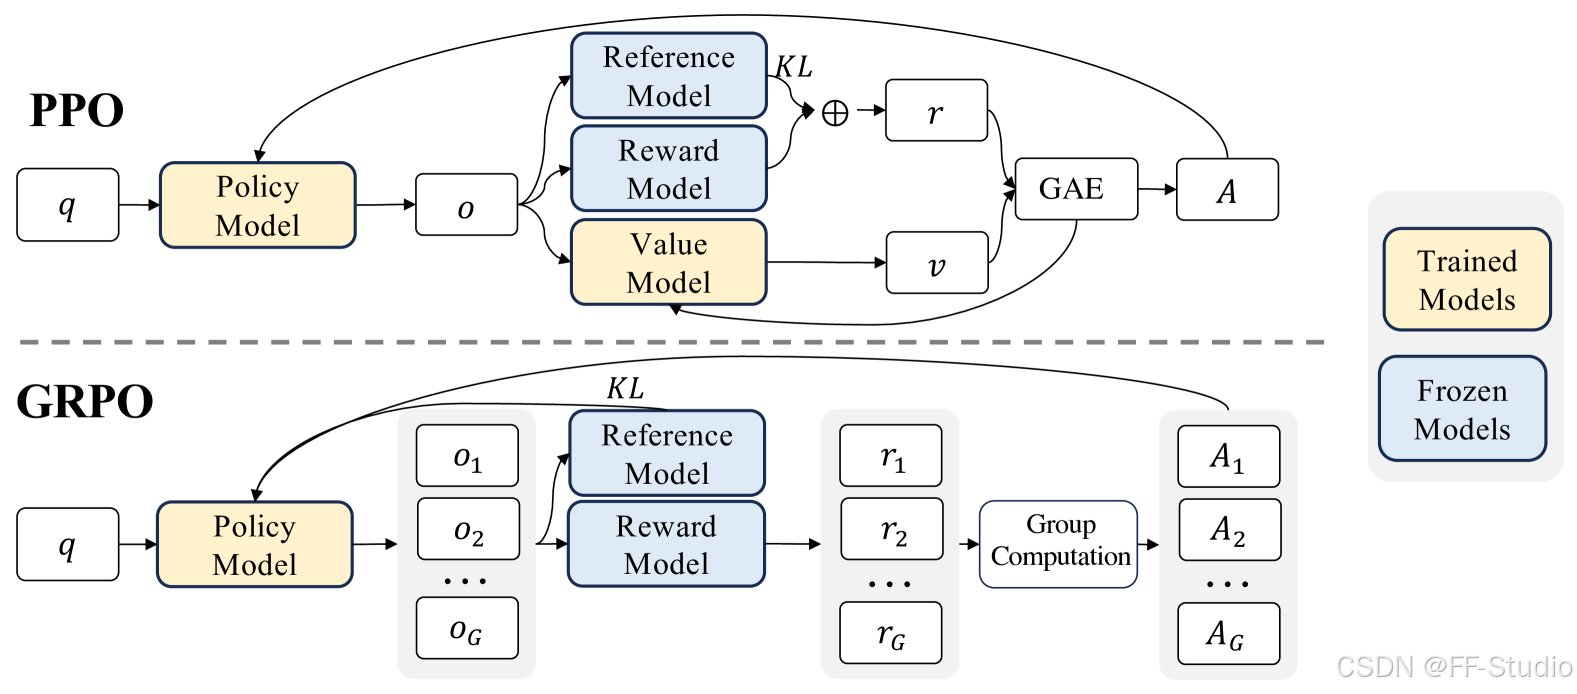
\includegraphics[width=0.6\textwidth]{GRPO/PPOvsGRPO.png}
    \end{figure}
    \begin{columns}[T]
        \column{0.4\textwidth}
        \begin{block}{主要步骤}
            \begin{enumerate}
                \item 分组采样
                \item 奖励归一化
                \item 策略更新
            \end{enumerate}
        \end{block}
        \column{0.6\textwidth}
        \begin{block}{GRPO三大优势}
            \begin{itemize}
                \item 单网络架构:仅需策略网络
                \item 分组相对奖励:同一问题下进行多候选对比
                \item 内存效率提升:节省40\%显存
            \end{itemize}
        \end{block}
    \end{columns} 
\end{frame}

\begin{frame}[fragile]
    \frametitle{GRPO Trainer 参数设置}
    \begin{columns}[T]
        \column{0.55\textwidth}
        \begin{block}{Python代码示例}
            \begin{lstlisting}[basicstyle=\small]
from trl import GRPOConfig, GRPOTrainer

# 训练参数配置
training_args = GRPOConfig(
    output_dir="my_model",
    num_generations=4,
    max_completion_length=256,
    temperature=0.9,
    per_device_train_batch_size=4,
    logging_steps=10
)
            \end{lstlisting}
        \end{block}
        
        \column{0.45\textwidth}
        \begin{block}{核心参数解析}
            \begin{itemize}
                \item \textbf{生成样本数}: 每个问题生成4-8个回答对比(num\_generations)
                \item \textbf{最大补全长度}: 控制生成文本长度(max\_completion\_length)
                \item \textbf{温度参数}: 0.9平衡多样性与质量(temperature)
                \item \textbf{KL系数}: 0.04防止模型跑偏
                \item \textbf{批次大小}: 根据显存调整(per\_device\_train\_batch\_size)
            \end{itemize}
        \end{block}


    \end{columns}
\end{frame}

% ================ 第五部分:DeepSeek R1 ======================
\section{DeepSeek R1解读}

\begin{frame}[fragile]
    \frametitle{推理模板}
    \begin{lstlisting}[basicstyle=\small]
    system:用户与助手的对话。用户提出问题,助手解决问题。
    助手首先在脑海中思考推理过程,然后向用户提供答案。
    推理过程和答案分别用<reasoning></reasoning>和<answer></answer>标签包裹,
    即:<reasoning> 此处为推理过程 </reasoning> <answer> 此处为答案 </answer>。

    user:(提示词,用户的问题)

    assistant:(为空,等待模型预测)

    \end{lstlisting}
    
    \begin{block}{模板设计原则}
        为引导基础模型遵循指定指令,设计了简洁的推理模板,仅约束结构格式,避免内容偏见。
    \end{block}
    \begin{itemize}
        \item \textbf{模板结构}: 用户与助手的对话形式
        \item \textbf{推理过程}: 使用<reasoning></reasoning>标签包裹
        \item \textbf{最终答案}: 使用<answer></answer>标签包裹
        \item \textbf{设计特点}: 避免强制特定推理策略,观察模型自然进化
    \end{itemize}
\end{frame}

\begin{frame}
    \frametitle{奖励函数}
    \begin{block}{实现方式概述}
        每个奖励函数都有其特定的实现逻辑,通常通过对生成结果进行解析和比较来计算得分。
    \end{block}
    \begin{itemize}
        \item \textbf{正确性奖励函数}: 通过提取生成答案中的内容,与真实答案进行比较,返回相应的分数。
        \item \textbf{格式奖励函数}: 使用正则表达式检查生成答案是否符合预定格式,返回相应的分数。
    \end{itemize}
\end{frame}

\begin{frame}
    \frametitle{DeepSeek R1解读}
    \begin{columns}[T]
        \column{0.55\textwidth}
        % 这里可以添加解读内容
        \begin{block}{论文解读}
            \begin{itemize}
                \item \textbf{简化版Pipeline如图}: 实际Pipeline比较复杂(Checkpoint生成数据),R0虽然输出胡言乱语,但Reasoning数据质量足够(拒绝采样挑出来好的,也可以整理成人话,作为高质量数据集)。
                \item \textbf{RL与SFT交错}: RL:提升智力;SFT:增加知识量,规范格式。(现阶段)RL会让模型输出胡言乱语,SFT会让模型变笨。
                \item \textbf{小模型蒸馏有效}: 对小模型RL,不如用高质量Reasoning数据SFT。
            \end{itemize}
        \end{block}
        
        \column{0.45\textwidth}
        \begin{figure}
            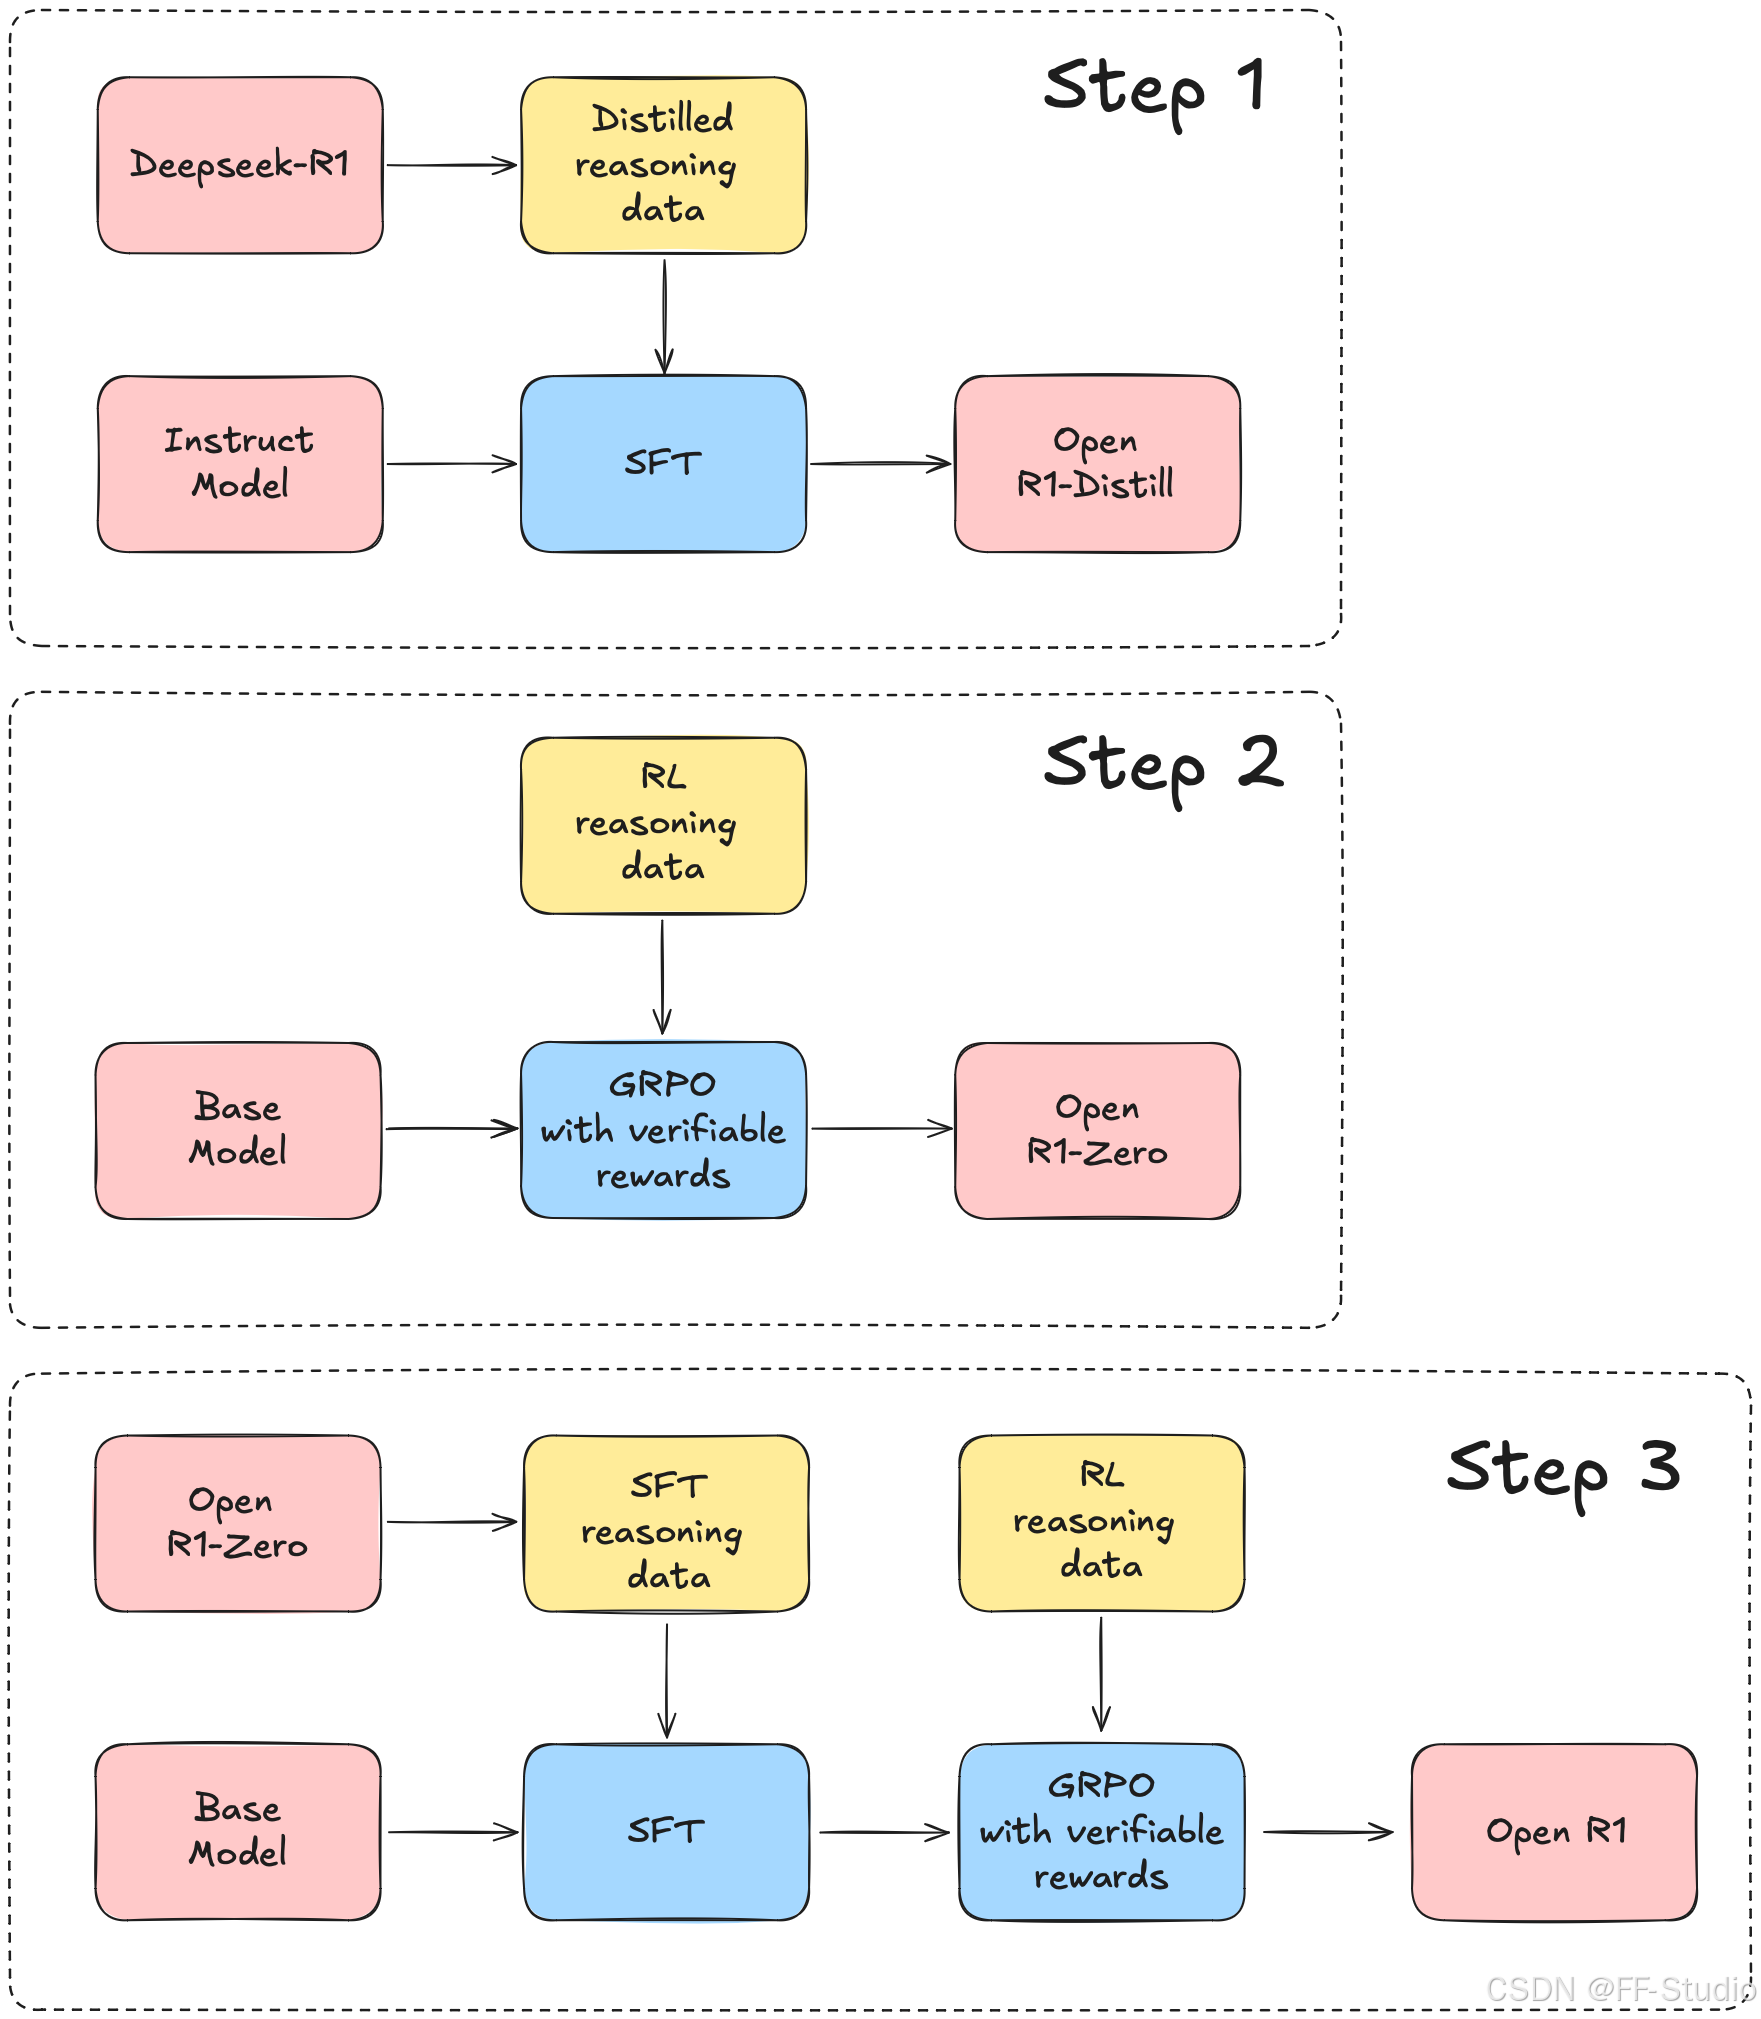
\includegraphics[width=0.9\textwidth]{GRPO/Open R1.png}
        \end{figure}
    \end{columns}
\end{frame}

% =================== 参考文献 ====================
\begin{frame}
    \frametitle{参考文献}
    {\small
    \begin{itemize}
        \item \href{https://arxiv.org/abs/2501.12948}{DeepSeek R1 论文《DeepSeek-R1: Incentivizing Reasoning Capability in LLMs via Reinforcement Learning》}
        \item \href{https://blog.csdn.net/qq_38961840/article/details/145556531}{DeepSeek-R1 译文及论文笔记《DeepSeek-R1:通过强化学习激发大语言模型的推理能力》}
        \item \href{https://arxiv.org/abs/2402.03300}{GRPO论文《DeepSeekMath: Pushing the Limits of Mathematical Reasoning in Open Language Models》}
        \item \href{https://blog.csdn.net/qq_38961840/article/details/145384346}{GRPO译文《DeepSeekMath: 推动开放语言模型在数学推理能力上的极限》}
        \item \href{https://blog.csdn.net/qq_38961840/article/details/145384852}{【DeepSeek】一文详解GRPO算法——为什么能减少大模型训练资源?}
        \item \href{https://blog.csdn.net/qq_38961840/article/details/145387854}{【DeepSeek】LLM强化学习GRPO Trainer详解}
        \item \href{https://github.com/huggingface/open-r1}{Open R1 项目《A fully open reproduction of DeepSeek-R1》}
        \item \href{https://blog.csdn.net/qq_38961840/article/details/145388142}{【DeepSeek】复现DeepSeek R1?快来看这个Open R1项目实践指南~}
        \item \href{https://blog.csdn.net/qq_38961840/article/details/145559997}{【解惑】Steps、Epochs、Batchsize?梯度累计步数、样本数?他们有什么关系?}
    \end{itemize}
    }
\end{frame}

\end{document}
